\documentclass{standalone}
\usepackage{tikz}
\usetikzlibrary{math, arrows, positioning}

\tikzstyle{node}= [circle, fill, minimum size=4pt,inner sep=0pt, outer sep=0pt]
\tikzstyle{node input}= [circle, fill, minimum size=4pt,inner sep=0pt, outer sep=0pt, pin={[pin edge={latex'-,black}]left:}]
\tikzstyle{node output}= [circle, fill, minimum size=4pt,inner sep=0pt, outer sep=0pt, pin={[pin edge={-latex',black}]right:}]
\tikzstyle{multiplier} = [circle, draw, inner sep=-1pt, font={${\times}$}]

\makeatletter
\long\def\ifnodedefined#1#2#3{%
	\@ifundefined{pgf@sh@ns@#1}{#3}{#2}%
}
\makeatother


\begin{document}
	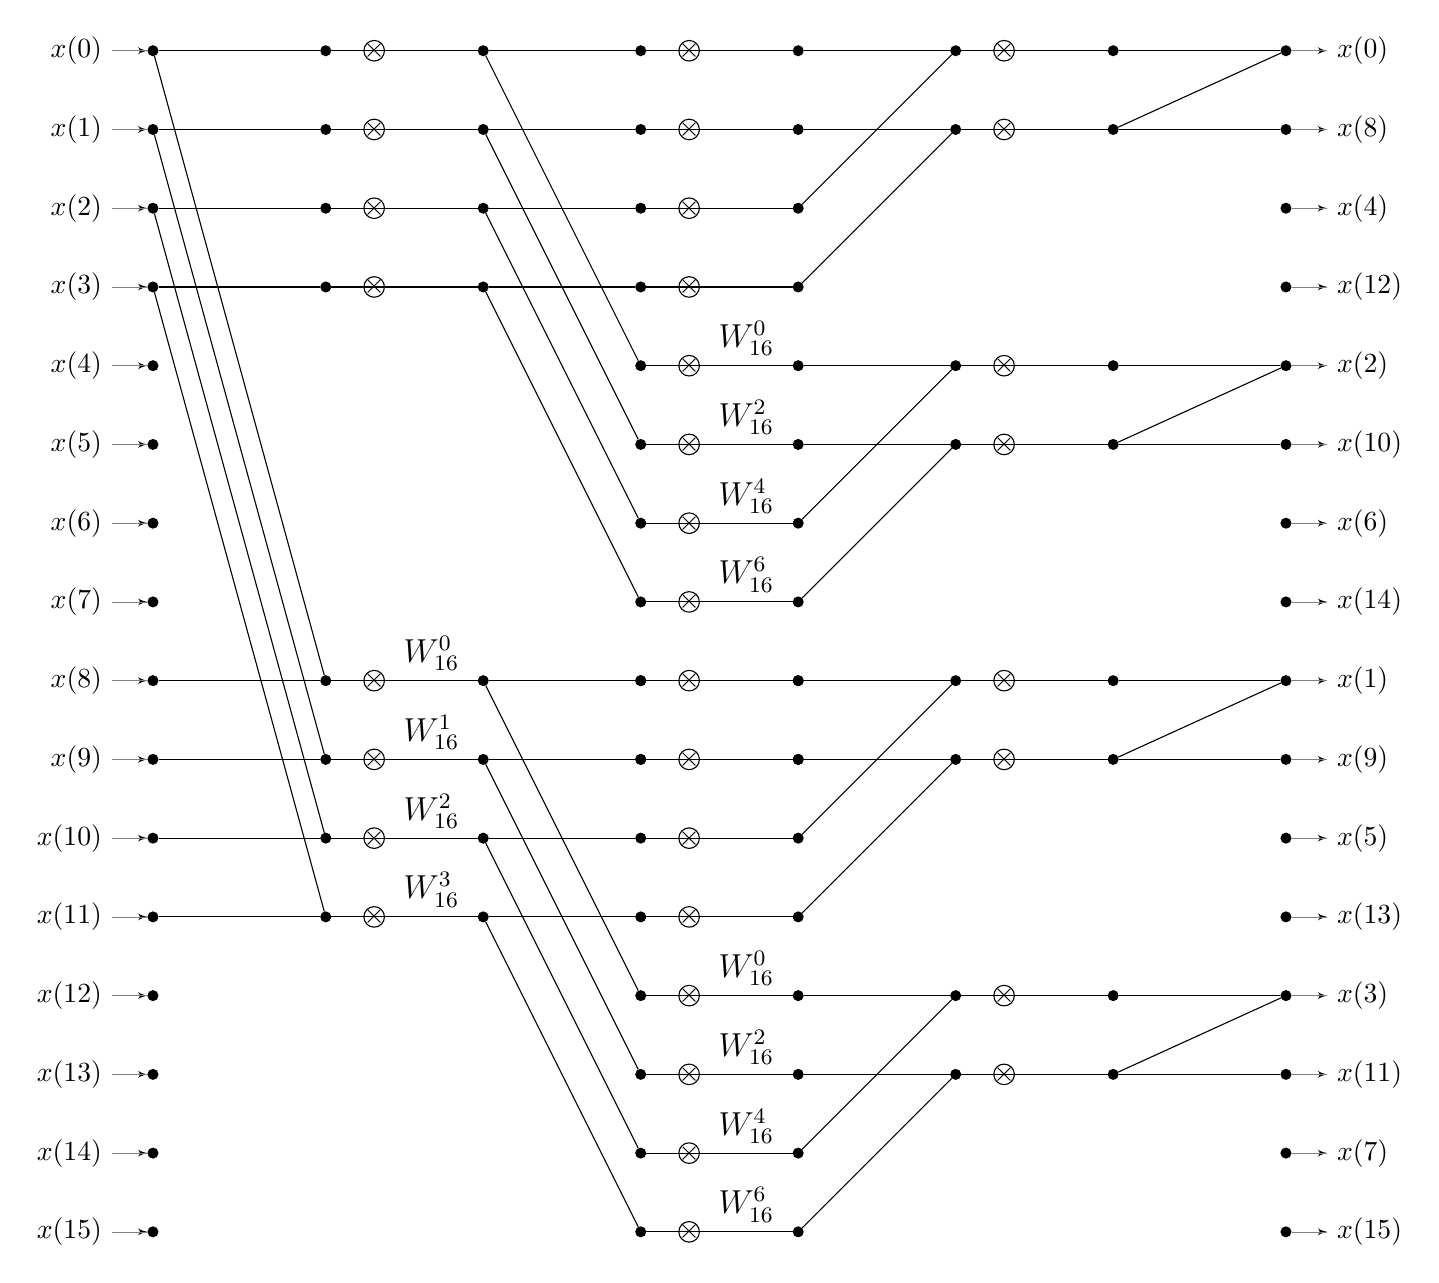
\begin{tikzpicture}

		% draw main points
		%% draw inputs
		\foreach \y in {0, ..., 15}
		{
			\node[node input, pin={[pin edge]left:$x(\y)$}] (point-0-\y) at (0, -\y) {};
		}
	
		%% draw grid-points
		\foreach \y in {0, ..., 15} {
			\foreach \x in {1, ..., 6} {
				\tikzmath{
					integer \xpos;
					\xpos = \x * 2;
				}
				
				\node[right=\xpos of point-0-\y] (grid-\x-\y) {};
			}
		}
	
		%% draw outputs
		\foreach \y / \result in {0/0, 1/8, 2/4, 3/12, 4/2, 5/10, 6/6, 7/14, 8/1, 9/9, 10/5, 11/13, 12/3, 13/11, 14/7, 15/15}
		{
			\node[node output, pin={[pin edge]right:$x(\result)$}, right=2 of grid-6-\y] (point-7-\y) {};
		}
	
		
		% draw points between input and output
		\foreach \y in {0, 1} {
			\foreach \x in {1, ..., 6} {
				\tikzmath{
					integer \xpos;
					\xpos = \x * 2;
				}
				
				\node[node] (point-\x-\y) at (grid-\x-\y) {};
			}
		}
	
		\foreach \y in {2, 3, 8, 9, 10, 11} {
			\foreach \x in {1, ..., 4} {
				\tikzmath{
					integer \xpos;
					\xpos = \x * 2;
				}
				
				\node[node] (point-\x-\y) at (grid-\x-\y) {};
			}
		}
	
		\foreach \y in {4, 5, 8, 9, 12, 13} {
			\foreach \x in {3, ..., 6} {
				\tikzmath{
					integer \xpos;
					\xpos = \x * 2;
				}
				
				\node[node] (point-\x-\y) at (grid-\x-\y) {};
			}
		}
	
		\foreach \y in {6, 7, 14, 15} {
			\foreach \x in {3, ..., 4} {
				\tikzmath{
					integer \xpos;
					\xpos = \x * 2;
				}
				
				\node[node] (point-\x-\y) at (grid-\x-\y) {};
			}
		}
	
		
		% draw operators
		\foreach \y in {0, ..., 15} {
			\foreach \x in {1, 3, 5} {
				\tikzmath{
					integer \xpos;
					\xpos = \x * 2;
				}
				
				\ifnodedefined{point-\x-\y}{
					\node[multiplier, right=10px of grid-\x-\y] (operator-\x-\y) {};
				}{}
			}
		}
	
	
		% draw verical lines
		\foreach \y in {0, ..., 15} {
			\tikzmath{
				integer \v;
				\v = \y - 1;
			}
			
			\ifnodedefined{point-6-\y}{
				\ifnodedefined{point-6-\v}{
					\path (point-6-\y) edge[-] (point-7-\v);
				}{}
			}{}
		}
	
		\foreach \y in {0, ..., 15} {
			\tikzmath{
				integer \v;
				\v = \y - 2;
			}
			
			\ifnodedefined{point-5-\v}{
				\path (point-4-\y) edge[-] (point-5-\v);
			}{}
		}
	
		\foreach \y in {0, ..., 15} {
			\tikzmath{
				integer \v;
				\v = \y + 4;
			}
			
			\ifnodedefined{point-2-\y}{
				\path (point-2-\y) edge[-] (point-3-\v);
			}{}
		}
	
		\foreach \y in {0, ..., 15} {
			\tikzmath{
				integer \v;
				\v = \y + 8;
			}
			
			\ifnodedefined{point-1-\v}{
				\path (point-0-\y) edge[-] (point-1-\v);
			}{}
		}
	
	
		% draw coefficients
		\foreach \y in {4, 12} {
			\tikzmath{
				integer \ny;
				integer \nny;
				integer \nnny;
				\ny = \y + 1;
				\nny = \y + 2;
				\nnny = \y + 3;
			}
			
			\path (point-3-\y) edge[-] (operator-3-\y);
			\path (operator-3-\y) edge[-] node[above]{\large$W^0_{16}$} (point-4-\y);
			
			\path (point-3-\ny) edge[-] (operator-3-\ny);
			\path (operator-3-\ny) edge[-] node[above]{\large$W^2_{16}$} (point-4-\ny);
			
			\path (point-3-\nny) edge[-] (operator-3-\nny);
			\path (operator-3-\nny) edge[-] node[above]{\large$W^4_{16}$} (point-4-\nny);
			
			\path (point-3-\nnny) edge[-] (operator-3-\nnny);
			\path (operator-3-\nnny) edge[-] node[above]{\large$W^6_{16}$} (point-4-\nnny);
		}
	
		\foreach \y in {8} {
			\tikzmath{
				integer \ny;
				integer \nny;
				integer \nnny;
				\ny = \y + 1;
				\nny = \y + 2;
				\nnny = \y + 3;
			}
			
			\path (point-1-\y) edge[-] (operator-1-\y);
			\path (operator-1-\y) edge[-] node[above]{\large$W^0_{16}$} (point-2-\y);
			
			\path (point-1-\ny) edge[-] (operator-1-\ny);
			\path (operator-1-\ny) edge[-] node[above]{\large$W^1_{16}$} (point-2-\ny);
			
			\path (point-1-\nny) edge[-] (operator-1-\nny);
			\path (operator-1-\nny) edge[-] node[above]{\large$W^2_{16}$} (point-2-\nny);
			
			\path (point-1-\nnny) edge[-] (operator-1-\nnny);
			\path (operator-1-\nnny) edge[-] node[above]{\large$W^3_{16}$} (point-2-\nnny);
		}
	
	
		% draw horizontal lines
		\foreach \y in {0, ..., 15} {
			\foreach \x in {0, ..., 7} {
				\tikzmath{
					integer \nx;
					\nx = \x + 1;
				}
				
				\ifnodedefined{point-\x-\y}{
					\ifnodedefined{point-\nx-\y}{
						\path (point-\x-\y) edge[-] (point-\nx-\y);
					}{}
				}{}
			}
		}
		
	\end{tikzpicture}
\end{document}